\subsection{Forced vibration of SDOF structures}


\solution{5}
The maximum displacements and accelerations of a vibrating structure under sinusoidal excitation are obtained from the stationary or homogeneous solution to the differential equation,
\begin{align*}
m\ddot{u} + ku = F_0\sin(\Omega t + \varphi) \\
u(t) = \frac{F_0}{k}H\sin(\Omega t + \varphi - \Delta\varphi)
\end{align*}

where $H$ is known as the magnification factor and is equal to
$$
H = \frac{1}{\sqrt{(1-\gamma^2)^2 + 4\xi^2\gamma^2}} \quad ; \quad
\gamma = \frac{\Omega}{\omega} = \frac{T_{struct}}{T_{force}}
$$

From the solution to example 3 (a) we know that the period is $T=0.9$ seconds and the frequency is $\omega = 2\pi/T \approx 7rad/s$ and the lateral stiffness is $k=487KN/m$. The damping ratio is $\xi=5\%$.

The amplitude $F_0$ of the external force is computed from the amplitude of the ground acceleration and the moving mass of the structure
$$
F_0 = ma_{0} = \frac{Pa_0}{g} = \frac{100\cdot2}{10} = 20KN
$$

Finally, the maximum displacements will depend on the period $\Omega$ of the external force,
\begin{align*}
&u_0 = \frac{F_0}{k}H = \frac{20}{487}H = 0.041H\ m = 4.1H\ cm \\
&\ddot{u}_0 = \frac{F_0}{m}\gamma^2H = \Omega^2u_0
\end{align*}


When the period of the ground acceleration is $T_g=0.15s$, the maximum displacements and accelerations are
\begin{align*}
&\gamma = \frac{0.9}{0.15} = 9 \quad ; \quad
H = \frac{1}{\sqrt{(1-9^2)^2 + 4\cdot 0.05^2\cdot 9^2}} = \frac{1}{\sqrt{80^4 + \cdots}} = 0.00015 \\
&u_0 = 4.1\cdot 0.00015 = 0.00064 cm \\
&\ddot{u}_0 = \left(\frac{2\pi}{0.15}\right)^2 \cdot 0.00064 = 1.1cm\,s^{-2} = 0.011m\,s^{-2}
\end{align*}
This situation is \emph{mass dominated}, also known as \emph{vibration isolation}.

When the period of the ground acceleration is $T_g=0.9s$, the maximum values are
\begin{align*}
&\gamma = \frac{0.9}{0.9} = 1 \quad ; \quad
H = \frac{1}{\sqrt{(1-1^2)^2 + 4\cdot 0.05^2\cdot 1^2}} = \frac{1}{\sqrt{0 + 4\cdot 0.05^2}} = 10 \\
&u_0 = 4.1\cdot 10 = 41 cm \\
&\ddot{u}_0 = \left(\frac{2\pi}{0.9}\right)^2 \cdot 41 = 2000cm\,s^{-2} = 20m\,s^{-2}
\end{align*}
The \emph{resonance} situation is \emph{damping dominated}.

And for a period $T_g=5s$, the maximum values are
\begin{align*}
&\gamma = \frac{0.9}{5} = 0.18 \quad ; \quad
H = \frac{1}{\sqrt{(1-0.18^2)^2 + 4\cdot 0.05^2\cdot 0.18^2}} = 1.033 \\
&u_0 = 4.1\cdot 1.033 = 4.2 cm \\
&\ddot{u}_0 = \left(\frac{2\pi}{5}\right)^2 \cdot 4.2 = 6.6cm\,s^{-2} = 0.066m\,s^{-2}
\end{align*}
Which is a practically \emph{static} situation or \emph{stiffness dominated}.



\solution{6}
When the building is hit by the helicopter, the impulse or linear momentum is preserved. To compute the linear momentum of the building, we need to know the equivalent mass and we can use the Rayleigh's method for that purpose. As it is suggested, we will use a linear shape function
\begin{align*}
&u = u_0\psi \quad ; \quad \psi = \frac{z}{h} \\
&m = \int_0^h \rho A\psi^2dz = \rho A\int_0^h\frac{z^2}{h^2}dz = \frac{1}{3}\rho Ah = \frac{1}{3} 1500 \cdot 400 \cdot 100 = \\
& \pushright{= 2\cdot 10^7N = 2\cdot 10^6Kg}
\end{align*}

The impulse of the helicopter is
$$
I = (mv)_{helicopter} = 10^4 \cdot 30 = 3\cdot 10^5 Kg\,m\,s^-1
$$
which is transferred to the building. Then, the maximum deflection at the top of the building is inferred
\begin{align*}
&\dot{u}_0 = \frac{I}{m} \quad \rightarrow \quad u_0 = \frac{I}{m\omega} \\
&\omega = \frac{2\pi}{T} = \frac{2\pi}{5} = 1.25rad\,s^{-1} \\
&u_0 = \frac{3\cdot 10^5}{2\cdot 10^6\cdot 1.25} = 0.12m = 12cm
\end{align*}



\solution{7}
Now, the building from example 6 is exposed to sudden wind gust. In that case dynamics of the  structure are defined by a \emph{mass spring damper} system under a constant force suddenly applied.The maximum amplitude is governed by the stationary or homogeneous solution to the differential equation
\begin{align*}
m\ddot{u} + c + ku = F_0 \\
u(t) = \frac{F_0}{k}(1 -e^{\xi\omega t}\cos(\omega t))
\end{align*}

First of all, we need to determine the equivalent lateral force using the Rayleigh's method from the wind pressure $p_W$, using the same shape function $\psi$ from example 6,
\begin{align*}
F_0 = \int_0^h p_W\psi dz = \int_0^h \left(0.3 + (1-0.3)\frac{z}{h}\right)\frac{z}{h}dz = \left(\frac{0.3}{2} + \frac{0.7}{3}\right)h = \\
= \left(\frac{0.3}{2} + \frac{0.7}{3}\right)100 = 38.3KN
\end{align*}

The stiffness of the building can be estimated from the equivalent mass and the given period of the building
$$
k = \omega^2m = \left(\frac{2\pi}{T}\right)^2m = \left(\frac{2\pi}{5}\right)^2 2\cdot 10^6 = 3.125\cdot 10^6 N/m = 3125KN/m
$$

Finally, the maximum displacement is obtained from the equation of motion
$$
u_{max} = \frac{F_0}{k}(1+1) = \frac{38.3}{3125}2 = 0.025m = 2.5cm
$$



\solution{8}
The motion of the mass released from a given height and attached to a cable has two parts. Firstly, a free fall. Secondly, a vibration. The velocity at the end of the free fall is
$$
\frac{1}{2}m\dot{u}_0^2 = mgl \quad \rightarrow \quad \dot{u}_0 = \sqrt{gl}
$$

And the vibration is described by a sudden force suddenly applied; the external force $F_0$ is generated by the gravity weight $mg$ and the stresses in the cable are obtained from elastic analysis. The same equations of example 7 can be applied here. Neglecting damping,
$$
u(t) = \frac{F_0}{k}(1 -\cos(\omega t))
$$

And the maximum displacement $u$ and stress $\sigma$ are
\begin{align*}
&u_{max} = \frac{F_0}{k}2 = 2\frac{mg}{EA} \\
&\sigma_{max} = E\varepsilon_{max} = E\frac{u_{max}}{l} = 2\frac{mg}{Al}
\end{align*}



\solution{9}
In that case, the magnitude of the external force $P=1KN$ is not varying with time, but moving with constant speed $v=10m/s$. The Rayleigh's method allow us to compute the equivalent force applied as a function of time. For that purpose, we choose a periodic shape function $\psi$ satisfying the kinematic boundary conditions
\begin{align*}
&\psi = \sin\left(\frac{\pi x}{l}\right) \\
&F = P\psi(x) = P\psi(vt) = P\sin\left(\frac{\pi vt}{l}\right)
\end{align*}
thus, the equivalent period of the external excitation is $\Omega = \pi v/l = 1\,rad\cdot s^{-1}$.

The mechanical properties of the section are
\begin{align*}
&A = 0.5m^2 \\
&I = \frac{1}{12}0.5^3 = \frac{0.125}{12} \approx 0.01 m^4\\
&E = 14GPa
\end{align*}

Now, the equivalent mass and stiffness can be computed with the Rayleigh's method,
\begin{align*}
&m = \int_0^l \rho A\psi^2dx = \int_0^l \rho A\sin^2\left(\frac{\pi x}{l}\right)dx = \frac{\rho Al}{2} = \\
& \pushright{= \frac{2800 \cdot 0.5 \cdot 10\pi}{2} = 7000\pi Kg = 7\pi Tn} \\
&k = \int_0^l EI\psi''^2dx = \int_0^l EI\left(-\left(\frac{\pi}{l}\right)^2\sin\left(\frac{\pi x}{l}\right)\right)^2dx = \frac{EI\pi^4}{2l^3} = \qquad \\
& \pushright{= \frac{14\cdot 10^6 \cdot 0.01 \cdot \pi^4}{2 \cdot (10\pi)^3} =
70\pi KN/m}
\end{align*}
and the frequency is
$$
\omega = \sqrt{\frac{k}{m}} = \sqrt{\frac{70\pi}{7\pi}} = \sqrt{10} = 3.16\,rad\cdot s^{-1}
$$

Finally, the structural response is obtained following the same steps from example 5, a structure under periodic loading. The deflection depends on the dynamic magnification factor $H$ and assuming a small damping ratio,
\begin{align*}
&\gamma = \frac{\Omega}{\omega} = \frac{\pi v}{l\omega} \\
&H = \frac{1}{\sqrt{\left(1-\frac{\pi^2v^2}{l^2\omega^2}\right)^2 + 4\xi^2\frac{\pi^2v^2}{l^2\omega^2}}} \approx \frac{1}{1-\frac{\pi^2v^2}{l^2\omega^2}} = \frac{l^2\omega^2}{l^2\omega^2-\pi^2v^2} = \qquad \\
&\pushright{= \frac{10^2\cdot\pi^2\cdot 3.16^2}{10^2\cdot\pi^2\cdot 3.16^2 - 10^2\cdot\pi^2}
= \frac{10}{10-1} = 1.11}
\end{align*}

Then, the deflection of the beam as a function of time is
$$
u = \frac{P}{k}H\sin(\Omega t) = \frac{1}{70\pi}1.11\sin(t) = 0.005\sin(t)\,m = 0.5\sin(t)\,cm
$$

And the maximum bending moment at the centre section is
$$
M_{max} = \frac{Pl}{4}H = \frac{1 \cdot 10\pi}{4}1.11 = 8.7\,KNm
$$



\solution{10}
A transient walking force is a periodic loading with piecewise definition. Hence, two approaches may be followed. The first one consist on supperposing the solutions of the piecewise excitating force. The solution will be analytical and piecewise, but restricted to that function. The second approach consist on approximating the pulse by a Fourier series. There will be a truncation error, but the procedure is valid for any arbitrary pulse.

\paragraph{Pre computed Fourier terms}
Each component of a Fourier series is also known ar harmonic. For a half sine activity, the amplitude of the first harmonics is

\begin{center}
\begin{tabular}{|l|c|cccc|}
    \hline
    Activity & $\alpha$ & $F_1/mg$ & $F_2/mg$ & $F_3/mg$ & $F_4/mg$ \\ \hline
    Walking  &    2/3   &   1.29   &   0.16   &   0.13   &   0.04   \\
    Exercise &    1/2   &   1.57   &   0.67   &   0.00   &   0.13   \\
    Jumping  &    1/3   &   1.80   &   1.29   &   0.67   &   0.16   \\
    High jumping & 1/4  &   1.89   &   1.57   &   1.13   &   0.67   \\ \hline
\end{tabular}
\end{center}


\paragraph{Fourier series}
Most commonly, Fourier series are expressed as a linear combination of $\sin$ and $\cos$,
$$
F(t) \approx \frac{a_0}{2} + \sum_{n=0}^{\infty} \left(a_n\cos(n\Omega t) + b_n\sin(n\Omega t)\right)
$$
with
\begin{align*}
a_0 &= \frac{2}{T}\int_{0}^{T} F(t) dt \\
a_n &= \frac{2}{T}\int_{0}^{T} F(t) \cos(n\Omega t) dt \\
b_n &= \frac{2}{T}\int_{0}^{T} F(t) \sin(n\Omega t) dt \\
\end{align*}

An alternative form is to compute the combination of the trigonometric functions as
$$
F(t) \approx F_0 + \sum_{n=0}^{\infty} F_n\sin(n\Omega t + \phi_n)
$$
with
\begin{align*}
&F_0 = \frac{a_0}{2} \\
&F_n = \sqrt{a_n^2 + b_n^2} \\
&\tan\phi_n = \frac{b_n}{a_n} \\
\end{align*}


\begin{center}
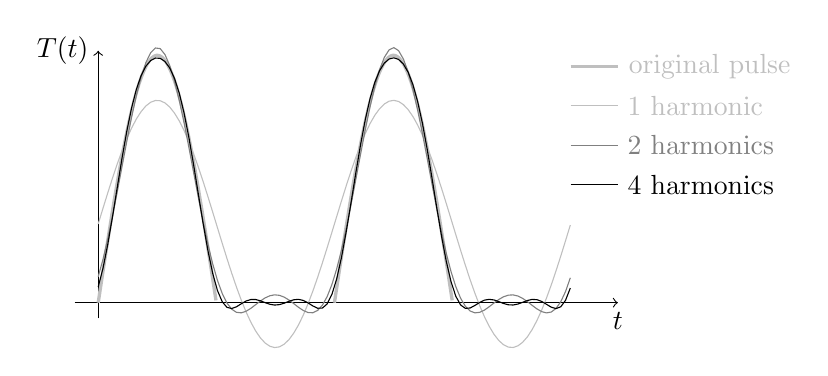
\begin{tikzpicture}[domain=0:2, xscale=3, samples=100]
    \draw[->] (-0.1,0) -- (2.2,0) node[below] {$t$};
    \draw[->] (0,-0.2) -- (0,3.2) node[left] {$T(t)$};

    % \x r means to convert '\x' from degrees to radians:
    \draw[very thick,lightgray,domain=0:0.5] plot (\x,{pi*sin(2*pi*\x r)});
    \draw[very thick,lightgray,domain=1:1.5] plot (\x,{pi*sin(2*pi*\x r)});
    \draw[lightgray] plot (\x,{1+1.57*sin(2*pi*\x r)});
    \draw[gray] plot (\x,{1+1.57*sin(2*pi*\x r)-0.67*cos(4*pi*\x r)});
    \draw[black] plot (\x,{1+1.57*sin(2*pi*\x r)-0.67*cos(4*pi*\x r)-0.13*cos(8*pi*\x r)});

    \draw[very thick,lightgray] (2,3)   -- +(.2,0) node[right] {original pulse};
    \draw[lightgray]            (2,2.5) -- +(.2,0) node[right] {1 harmonic};
    \draw[gray]                 (2,2)   -- +(.2,0) node[right] {2 harmonics};
    \draw[black]                (2,1.5) -- +(.2,0) node[right] {4 harmonics};
\end{tikzpicture}
\end{center}


\paragraph{Discrete Fourier series}


